\onehalfspacing
\section{Đề số 33}

\begin{bt} 
	\hfill
	\begin{enumerate}[a.]
		\item Tính giá trị $A=1000-\left\{(-5)^3 \cdot(-2)^3-11 \cdot\left[7^2-5 \cdot 2^3+8\left(11^2-121\right)\right]\right\}$
		\item Tìm $x$ biết $\left(3-\frac{9}{10}-|x+2|\right):\left(\frac{19}{10}-1-\frac{2}{5}\right)+\frac{4}{5}=1$
		\item Tìm $x$ thỏa mãn $|x-10|^{10}+|x-11|^{11}=1$
	\end{enumerate}
	\loigiai{
		\begin{enumerate}
			\item $\text {Ta có: }\\[5px] 
			A =1000-\{(-125) \cdot(-8)-11 \cdot[49-40+8 \cdot(121-121)]\} \\[5px]
			=1000-[1000-11 \cdot(9+8 \cdot 0)] \\[5px]
			=1000-(1000-11 \cdot 9) \\[5px]
			=99$
			\item Ta có:\\[5px]
			$\left(3-\frac{9}{10}-|x+2|\right):\left(\frac{19}{10}-1-\frac{2}{5}\right)+\frac{4}{5}=1 \\[5px]
			\Leftrightarrow\left(\frac{30}{10}-\frac{9}{10}-|x+2|\right):\left(\frac{19}{10}-\frac{10}{10}-\frac{4}{10}\right)=1-\frac{4}{5} \\[5px]
			\Leftrightarrow\left(\frac{21}{10}-|x+2|\right): \frac{5}{10}=\frac{1}{5} \\[5px]
			\Leftrightarrow \frac{21}{10}-|x+2|=\frac{1}{5} \cdot \frac{5}{10}=\frac{1}{10} \\[5px]
			\Leftrightarrow|x+2|=\frac{21}{10}-\frac{1}{10}=2 \\[5px]
			\Leftrightarrow x+2=-2 ; 2 \\[5px]
			\Leftrightarrow x=-4 ; 0 \\[5px]
			\text {Vậy } x=0 ;-4$
			\item - Nếu $x>11$ hoặc $x<10$ thì $x-10>1$ hoặc $x-11<-1$.\\[5px] 
			Suy ra $|x-10|>1 ;|x-11|>1$ (loại)\\[5px]
			- Nếu $10<\mathrm{x}<11$ thì $0<\mathrm{x}-10<1,0<11-\mathrm{x}<1$. Suy ra $|x-10|<1 ;|x-11|<1$. Do đó $|x-10|^{10}<|x-10|=x-10 ;|x-11|^{11}=|11-x|^{11}<|11-x|=11-x$\\[5px]
			Suy ra $|x-10|^{10}+|x-11|^{11}<x-10+11-x=1$ (loại)\\[5px]
			- Nếu $x=10$ hoặc $x=11$ thỏa mãn\\[5px]
			Vậy $x=10 ; 11$
		\end{enumerate}
	} 
\end{bt}

\begin{bt}
	\hfill
	\begin{enumerate}[a.]
		\item Tìm hai số dương khác nhau $x$, $y$ biết rằng: Tổng, hiệu và tích của chúng lân lượt tỉ lệ nghịch với $35 ; 210$ và 12 .
		\item Cho a, b, c là các số thực khác 0 . Tìm các số thực $\mathrm{x}, \mathrm{y}, \mathrm{z}$ khác 0 thoả mãn:
		$$
		\frac{x y}{a y+b x}=\frac{y z}{b z+c y}=\frac{z x}{c x+a z}=\frac{x^2+y^2+z^2}{a^2+b^2+c^2}
		$$
	\end{enumerate}
	\loigiai{
		\begin{enumerate}
			\item Gọi hai số phải tìm là $\mathrm{x}$ và $\mathrm{y}(\mathrm{x}>0, \mathrm{y}>0$ và $\mathrm{x} \neq \mathrm{y})$\\[5px]
			Theo đề bài ta có: 35. $(x+y)=210 .(x-y)=12 x . y$\\[5px]
			Chia các tích trên cho $\mathrm{BCNN}$ của $35,210,12$ là 420 ta được:\\[5px]
			$\frac{35 \cdot(x+y)}{420}=\frac{210(x-y)}{420}=\frac{12 x y}{420}$\\[5px] 
			hay $\frac{x+y}{12}=\frac{x-y}{2}=\frac{x y}{35}$ (1)\\[5px]
			Theo tính chất của dãy tỉ số bằng nhau ta có:\\[5px]
			$\frac{x+y}{12}=\frac{x-y}{2}=\frac{(x+y)+(x-y)}{12+2}=\frac{(x+y)-(x-y)}{12-2} \\[5px]
			\Leftrightarrow \frac{x+y}{12}=\frac{x-y}{2}=\frac{x}{7}=\frac{y}{5}(2)$\\[5px]
			Từ (1) và (2) ta có: $\frac{x y}{35}=\frac{x}{7}=\frac{y}{5}=\frac{x y}{7 y}=\frac{x y}{5 x}$\\[5px]
			$\text {Vì } x>0 ; y>0 \text { nên } 7 y=35\\[5px] \Rightarrow y=5 ; 5 x=35 \Rightarrow x=7$\\[5px]
			Vậy hai số phải tìm là 7 và 5.
			\item Do x, y, z khác 0 nên $\frac{x y}{a y+b x}=\frac{y z}{b z+c y}=\frac{z x}{c x+a z}\\[5px] \Rightarrow \frac{z x y}{a y z+b x z}=\frac{x y z}{b z x+c y x}=\frac{y z x}{c x y+a z y}$\\[5px]
			Suy ra $a y z+b x z=b z x+c y x=c x y+a z y \Rightarrow a z=c x, b x=a y$\\[5px]
			Do đó $\frac{x}{a}=\frac{z}{c}, \frac{x}{a}=\frac{y}{b} \Rightarrow \frac{x}{a}=\frac{y}{b}=\frac{z}{c}=t \Rightarrow x=a t, \mathrm{y}=b t, z=c t, t \neq 0$\\[5px]
			Ta có $\frac{x y}{a y+b x}=\frac{x^2+y^2+z^2}{a^2+b^2+c^2} \Rightarrow \frac{a t . b t}{a b t+b a t}=\frac{a^2 t^2+b^2 t^2+c^2 t^2}{a^2+b^2+c^2}$\\[5px]
			Suy ra $\frac{t}{2}=t^2 \Rightarrow t=\frac{1}{2}($ do $t \neq 0)$\\[5px]
			Vậy $x=\frac{a}{2}, \mathrm{y}=\frac{b}{2}, z=\frac{c}{2}$
		\end{enumerate}
	} 
\end{bt}

\begin{bt}
	\hfill 
	\begin{enumerate}[a.]
		\item Tìm $x$, y nguyên thoả mãn $3 x y-5=x^2+2 y$
		\item Tìm số có bốn chữ số $\overline{a b c d}$ thỏa mãn đồng thời hai điều kiện sau:
		\begin{enumerate}[i.]
			\item $\overline{a b}, \overline{a d}$ là hai số nguyên tố;
			\item $\overline{d b}+\mathrm{c}=\mathrm{b}^2+\mathrm{d}$.
		\end{enumerate}
	\end{enumerate}
	\loigiai{
		\begin{enumerate}
			\item Theo đề ta có $3 x y-2 y=x^2+5 \Rightarrow y(3 x-2)=x^2+5$\\[5px]
			Do $x, y$ nguyên nên suy ra $x^2+5$ chia hết cho $3 x-2$\\[5px]
			$\Rightarrow 9 .\left(x^2+5\right)$ chia hết cho $3 x-2$\\[5px]
			$\Rightarrow 9 \cdot x^2+45$ chia hết cho $3 x-2\\[5px] \Rightarrow 9 \cdot x^2-6 x+6 x-4+49$ chia hết cho $3 x-2$\\[5px]
			$\Rightarrow 3 x .(3 x-2)+2(3 x-2)+49$ chia hết cho $3 x-2$\\[5px]
			$\Rightarrow 49$ chia hết cho $3 x-2 \Rightarrow 3 x-2 \in\{-49 ;-7 ;-1 ; 1 ; 7 ; 49\}$\\[5px]
			$\Rightarrow 3 x \in\{-47 ;-5 ; 1 ; 3 ; 9 ; 51\} \Rightarrow x \in\{1 ; 3 ; 17\}$\\[5px]
			Thay $x$ lần lượt vào (1) ta được $y \in\{6 ; 2 ; 6\}$\\[5px]
			Vậy các cặp số $(x, y)$ là $(1 ; 6),(3 ; 2),(17 ; 6)$
			\item Do $\overline{a b} ; \overline{a d}$ là các số nguyên tố nên b và $\mathrm{d}$ lẻ khác 5 (1)\\[5px]
			Mặt khác từ điều kiện ii) ta có $9 \mathrm{~d}+\mathrm{c}=\mathrm{b}(\mathrm{b}-1)$ (2)\\[5px]
			Có $9 \mathrm{~d}+\mathrm{c} \geq 9$ nên từ (2) suy ra $b>3$ mà $b$ lẻ $\Rightarrow \mathrm{b}=7 ; 9$\\[5px]
			$+\mathrm{b}=7 \Rightarrow 9 \mathrm{~d}+\mathrm{c}=42 \Rightarrow 3<\mathrm{d} \leq 4$ trái với (1)\\[5px]
			$+\mathrm{b}=9 \Rightarrow 9 \mathrm{~d}+\mathrm{c}=72 \Rightarrow 6<\mathrm{d} \leq 8$ mà $\mathrm{d}$ lẻ $\Rightarrow \mathrm{d}=7$\\[5px] 
			Thay vào điều kiện (2) được $c=9$.\\[5px]
			Do $\bar{a} ; \overline{a 7}$ là các số nguyên tố nên a chỉ có thể nhận các giá trị tương ứng $1 ; 2 ; 5 ; 7 ; 8$ hoặc 1 ; $3 ; 4 ; 6 ; 9$.\\[5px] 
			Suy ra $a=1$ và $\overline{a b c d}=1997$, thử lại thấy đúng.
		\end{enumerate}
	} 
\end{bt}

\begin{bt}
	Cho tam giác $A B C$ có $\hat{B}<90^{\circ}$ và $\hat{B}=2 \hat{C}$. Trên tia đối của tia $\mathrm{BA}$ lấy điểm $\mathrm{E}$ sao cho $\mathrm{BE}=\mathrm{BH}$ (với $\mathrm{H}$ là chân đường vuông góc kẻ từ $\mathrm{A}$ đến $\mathrm{BC}$ ), đường thẳng $\mathrm{EH}$ cắt $\mathrm{AC}$ ở $\mathrm{D}$.
	\begin{enumerate}[a.]
		\item Chứng minh rằng: $\mathrm{DA}=\mathrm{DC}$.
		\item Chứng minh rằng: $\mathrm{AE}=\mathrm{HC}$.
	\end{enumerate}
	\loigiai{
		$$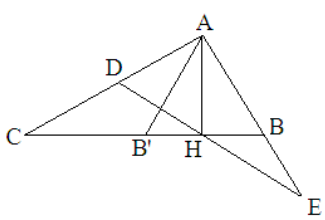
\includegraphics[width=0.4\textwidth]{33-4-lg.png}$$
		\begin{enumerate}
			\item Ta có $\triangle \mathrm{BEH}$ cân tại $\mathrm{B} \Rightarrow \angle \mathrm{BEH}=\angle \mathrm{BHE}$\\[5px]
			Ta có $\angle \mathrm{ABC}=$ 2. $\angle \mathrm{BHE}=$ 2. $\angle \mathrm{DHC}$ mà $\angle \mathrm{ABC}=2 . \angle \mathrm{ACB} \Rightarrow \angle \mathrm{DHC}=\angle \mathrm{DCH}(1)$\\[5px]
			Suy ra $\Delta \mathrm{DCH}$ cân tại $\mathrm{D}$ nên $\mathrm{DH}=\mathrm{DC}$\\[5px]
			Xét $\triangle \mathrm{ACH}: \angle \mathrm{CAH}+\angle \mathrm{DCH}=90^{\circ}, \angle \mathrm{CHD}+\angle \mathrm{DHA}=90^{\circ}$ (2)\\[5px]
			Từ (1), (2) suy ra $\angle \mathrm{DAH}=\angle \mathrm{DHA}$, do đó $\triangle \mathrm{DAH}$ cân tại $\mathrm{D}$, suy ra $\mathrm{DA}=\mathrm{DC}$.
			\item Lấy $\mathrm{B}^{\prime}$ đối xứng với $\mathrm{B}$ qua $\mathrm{H}$, suy ra $\triangle \mathrm{ABB}^{\prime}$ cân tại $\mathrm{A}\left(\mathrm{AH}\right.$ là trung trực của $\mathrm{BB}^{\prime}$ )\\[5px]
			$\Rightarrow \mathrm{AB}=\mathrm{AB}^{\prime}, \mathrm{B}^{\prime} \mathrm{H}=\mathrm{BH}, \angle \mathrm{AB}^{\prime} \mathrm{H}=\angle \mathrm{ABC}$\\[5px]
			Ta có $\angle \mathrm{AB}^{\prime} \mathrm{H}=\angle \mathrm{ABC}=$ 2. $\angle \mathrm{C}=\angle \mathrm{C}+\angle \mathrm{CAB}^{\prime}\\[5px] 
			\Rightarrow \angle \mathrm{C}=\angle \mathrm{CAB}^{\prime}$, do đó $\Delta \mathrm{B}^{\prime} \mathrm{AC}$ cân tại $\mathrm{B}^{\prime}$ nên $\mathrm{B}^{\prime} \mathrm{A}=\mathrm{B}^{\prime} \mathrm{C}$\\[5px]
			Vì $\mathrm{AB}<\mathrm{AC}$ nên $\mathrm{AB}^{\prime}=\mathrm{AB}<\mathrm{AC}$ nghĩa là $\mathrm{B}^{\prime}$ ở giữa $\mathrm{H}$ và $\mathrm{C}$ nên\\[5px]
			$\mathrm{HC}=\mathrm{HB}^{\prime}+\mathrm{B}^{\prime} \mathrm{C}=\mathrm{HB}+\mathrm{AB}^{\prime}=\mathrm{BE}+\mathrm{AB}=\mathrm{AE}$
		\end{enumerate}
	}
\end{bt}
